% !TEX TS-program = pdflatex
% !TEX encoding = UTF-8 Unicode
\documentclass[border=0mm]{standalone}
% packages
\usepackage{tikz}
\usetikzlibrary{patterns}
\usepackage{amsmath,amssymb}
\usepackage{bm}
\usepackage{pgfplots}
\pgfplotsset{compat=1.15}
% start document
\begin{document}
% generated by ROOT (CERN)
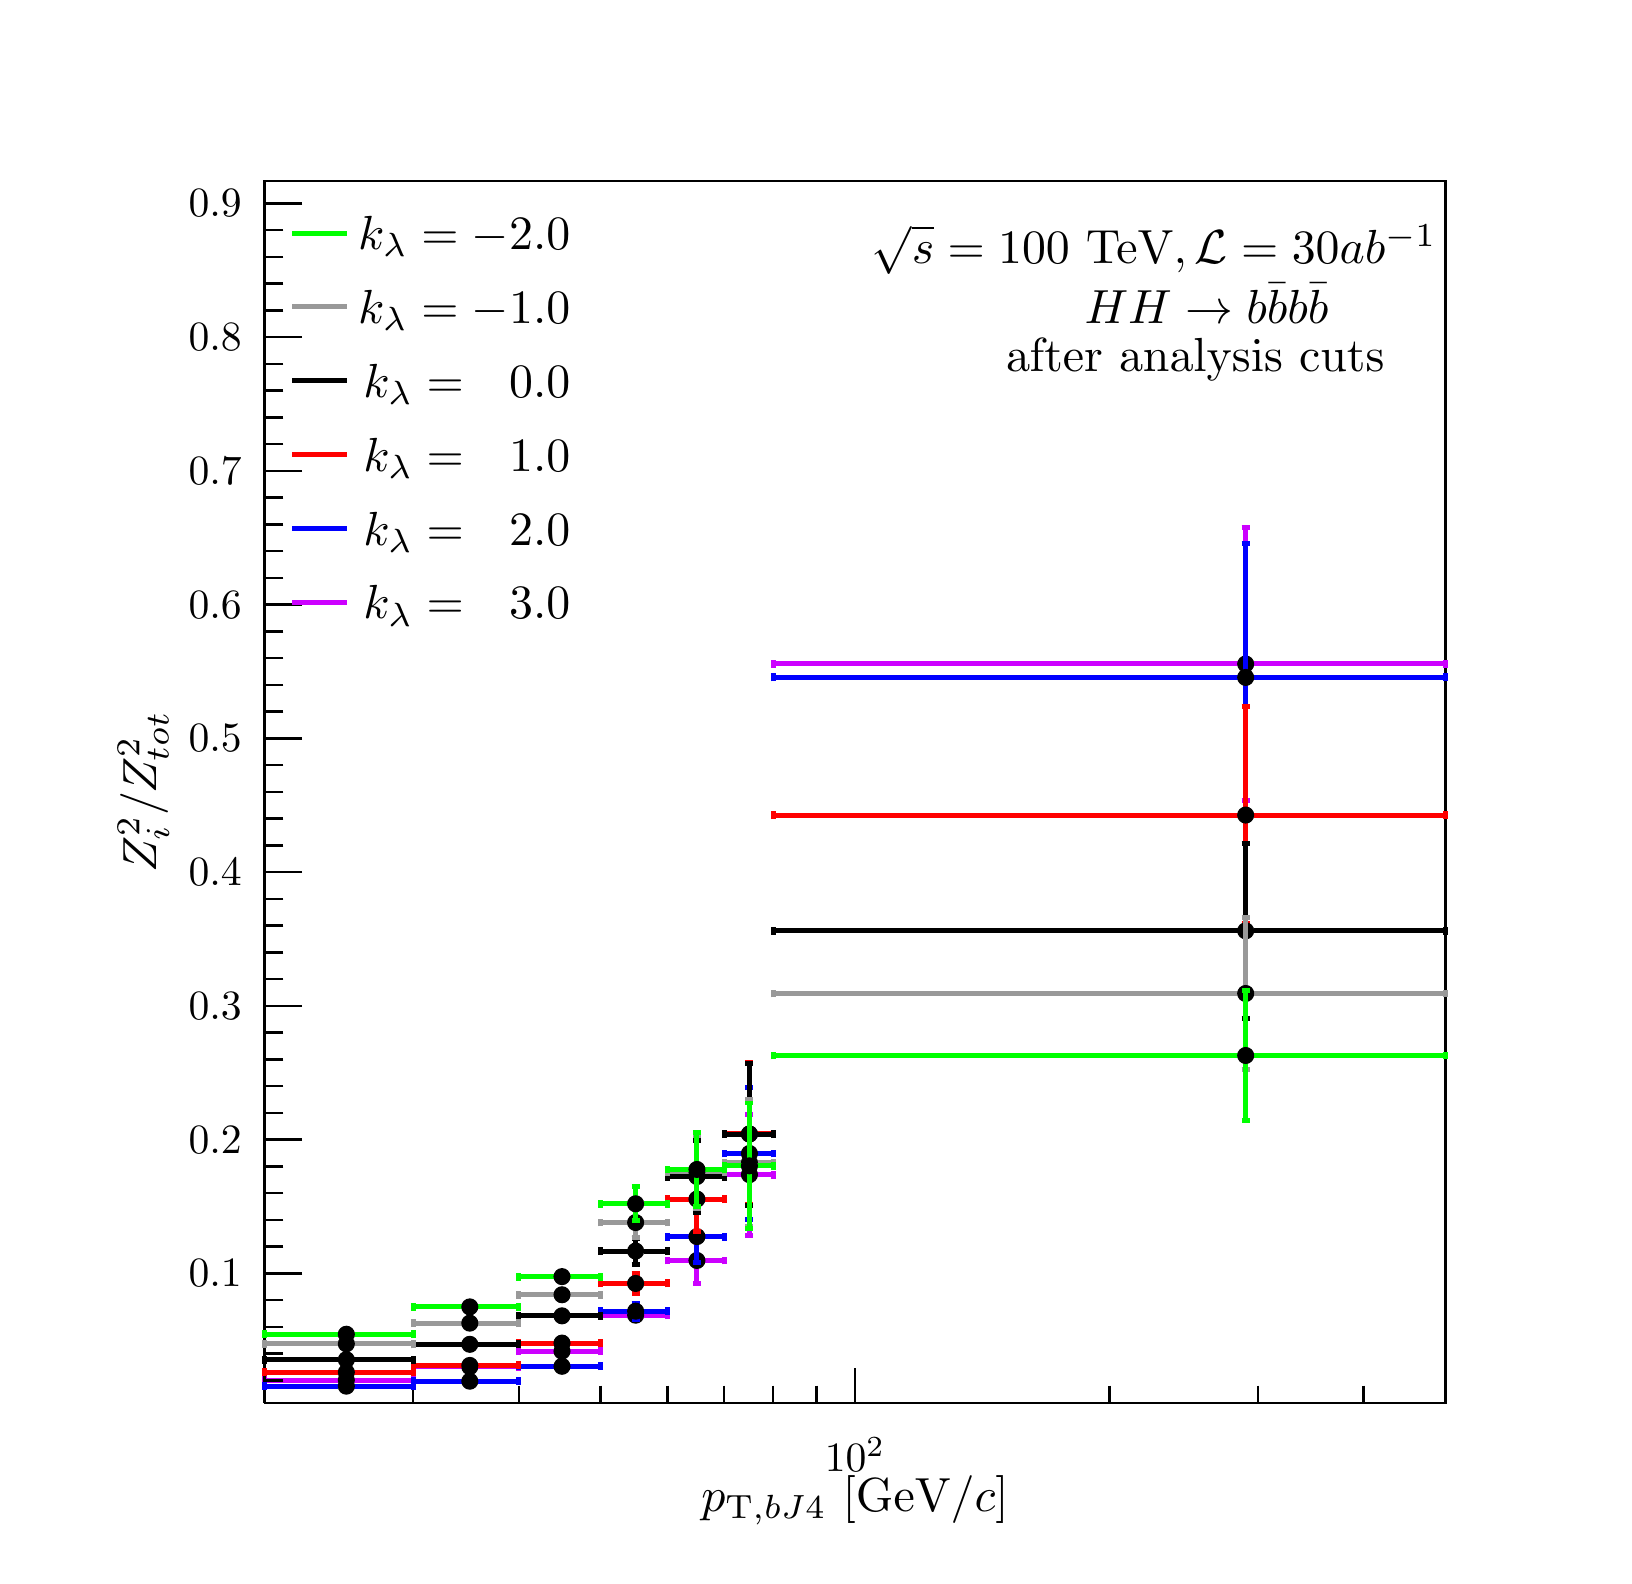
\begin{tikzpicture}
\pgfdeclareplotmark{cross} {
\pgfpathmoveto{\pgfpoint{-0.3\pgfplotmarksize}{\pgfplotmarksize}}
\pgfpathlineto{\pgfpoint{+0.3\pgfplotmarksize}{\pgfplotmarksize}}
\pgfpathlineto{\pgfpoint{+0.3\pgfplotmarksize}{0.3\pgfplotmarksize}}
\pgfpathlineto{\pgfpoint{+1\pgfplotmarksize}{0.3\pgfplotmarksize}}
\pgfpathlineto{\pgfpoint{+1\pgfplotmarksize}{-0.3\pgfplotmarksize}}
\pgfpathlineto{\pgfpoint{+0.3\pgfplotmarksize}{-0.3\pgfplotmarksize}}
\pgfpathlineto{\pgfpoint{+0.3\pgfplotmarksize}{-1.\pgfplotmarksize}}
\pgfpathlineto{\pgfpoint{-0.3\pgfplotmarksize}{-1.\pgfplotmarksize}}
\pgfpathlineto{\pgfpoint{-0.3\pgfplotmarksize}{-0.3\pgfplotmarksize}}
\pgfpathlineto{\pgfpoint{-1.\pgfplotmarksize}{-0.3\pgfplotmarksize}}
\pgfpathlineto{\pgfpoint{-1.\pgfplotmarksize}{0.3\pgfplotmarksize}}
\pgfpathlineto{\pgfpoint{-0.3\pgfplotmarksize}{0.3\pgfplotmarksize}}
\pgfpathclose
\pgfusepathqstroke
}
\pgfdeclareplotmark{cross*} {
\pgfpathmoveto{\pgfpoint{-0.3\pgfplotmarksize}{\pgfplotmarksize}}
\pgfpathlineto{\pgfpoint{+0.3\pgfplotmarksize}{\pgfplotmarksize}}
\pgfpathlineto{\pgfpoint{+0.3\pgfplotmarksize}{0.3\pgfplotmarksize}}
\pgfpathlineto{\pgfpoint{+1\pgfplotmarksize}{0.3\pgfplotmarksize}}
\pgfpathlineto{\pgfpoint{+1\pgfplotmarksize}{-0.3\pgfplotmarksize}}
\pgfpathlineto{\pgfpoint{+0.3\pgfplotmarksize}{-0.3\pgfplotmarksize}}
\pgfpathlineto{\pgfpoint{+0.3\pgfplotmarksize}{-1.\pgfplotmarksize}}
\pgfpathlineto{\pgfpoint{-0.3\pgfplotmarksize}{-1.\pgfplotmarksize}}
\pgfpathlineto{\pgfpoint{-0.3\pgfplotmarksize}{-0.3\pgfplotmarksize}}
\pgfpathlineto{\pgfpoint{-1.\pgfplotmarksize}{-0.3\pgfplotmarksize}}
\pgfpathlineto{\pgfpoint{-1.\pgfplotmarksize}{0.3\pgfplotmarksize}}
\pgfpathlineto{\pgfpoint{-0.3\pgfplotmarksize}{0.3\pgfplotmarksize}}
\pgfpathclose
\pgfusepathqfillstroke
}
\pgfdeclareplotmark{newstar} {
\pgfpathmoveto{\pgfqpoint{0pt}{\pgfplotmarksize}}
\pgfpathlineto{\pgfqpointpolar{44}{0.5\pgfplotmarksize}}
\pgfpathlineto{\pgfqpointpolar{18}{\pgfplotmarksize}}
\pgfpathlineto{\pgfqpointpolar{-20}{0.5\pgfplotmarksize}}
\pgfpathlineto{\pgfqpointpolar{-54}{\pgfplotmarksize}}
\pgfpathlineto{\pgfqpointpolar{-90}{0.5\pgfplotmarksize}}
\pgfpathlineto{\pgfqpointpolar{234}{\pgfplotmarksize}}
\pgfpathlineto{\pgfqpointpolar{198}{0.5\pgfplotmarksize}}
\pgfpathlineto{\pgfqpointpolar{162}{\pgfplotmarksize}}
\pgfpathlineto{\pgfqpointpolar{134}{0.5\pgfplotmarksize}}
\pgfpathclose
\pgfusepathqstroke
}
\pgfdeclareplotmark{newstar*} {
\pgfpathmoveto{\pgfqpoint{0pt}{\pgfplotmarksize}}
\pgfpathlineto{\pgfqpointpolar{44}{0.5\pgfplotmarksize}}
\pgfpathlineto{\pgfqpointpolar{18}{\pgfplotmarksize}}
\pgfpathlineto{\pgfqpointpolar{-20}{0.5\pgfplotmarksize}}
\pgfpathlineto{\pgfqpointpolar{-54}{\pgfplotmarksize}}
\pgfpathlineto{\pgfqpointpolar{-90}{0.5\pgfplotmarksize}}
\pgfpathlineto{\pgfqpointpolar{234}{\pgfplotmarksize}}
\pgfpathlineto{\pgfqpointpolar{198}{0.5\pgfplotmarksize}}
\pgfpathlineto{\pgfqpointpolar{162}{\pgfplotmarksize}}
\pgfpathlineto{\pgfqpointpolar{134}{0.5\pgfplotmarksize}}
\pgfpathclose
\pgfusepathqfillstroke
}
\definecolor{c}{rgb}{1,1,1};
\draw [color=c, fill=c] (0,0) rectangle (20,19.397);
\draw [color=c, fill=c] (3,1.9397) rectangle (18,17.4573);
\definecolor{c}{rgb}{0,0,0};
\draw [c,line width=0.9] (3,1.9397) -- (3,17.4573) -- (18,17.4573) -- (18,1.9397) -- (3,1.9397);
\definecolor{c}{rgb}{1,1,1};
\draw [color=c, fill=c] (3,1.9397) rectangle (18,17.4573);
\definecolor{c}{rgb}{0,0,0};
\draw [c,line width=0.9] (3,1.9397) -- (3,17.4573) -- (18,17.4573) -- (18,1.9397) -- (3,1.9397);
\definecolor{c}{rgb}{0.8,0,1};
\draw [c,line width=1.8] (3,2.22794) -- (3.93935,2.22794);
\draw [c,line width=1.8] (4.14035,2.22794) -- (4.88947,2.22794);
\draw [c,line width=1.8] (3,2.17769) -- (3,2.27819);
\draw [c,line width=1.8] (4.88947,2.17769) -- (4.88947,2.27819);
\definecolor{c}{rgb}{0,0,0};
\foreach \P in {(4.03985,2.22794)}{\draw[mark options={color=c,fill=c},mark size=2.882883pt,mark=*] plot coordinates {\P};}
\definecolor{c}{rgb}{0.8,0,1};
\draw [c,line width=1.8] (4.88947,2.39763) -- (5.50731,2.39763);
\draw [c,line width=1.8] (5.70832,2.39763) -- (6.23007,2.39763);
\draw [c,line width=1.8] (4.88947,2.34738) -- (4.88947,2.44788);
\draw [c,line width=1.8] (6.23007,2.34738) -- (6.23007,2.44788);
\definecolor{c}{rgb}{0,0,0};
\foreach \P in {(5.60782,2.39763)}{\draw[mark options={color=c,fill=c},mark size=2.882883pt,mark=*] plot coordinates {\P};}
\definecolor{c}{rgb}{0.8,0,1};
\draw [c,line width=1.8] (6.23007,2.59577) -- (6.67844,2.59577);
\draw [c,line width=1.8] (6.87945,2.59577) -- (7.26993,2.59577);
\draw [c,line width=1.8] (6.23007,2.54551) -- (6.23007,2.64602);
\draw [c,line width=1.8] (7.26993,2.54551) -- (7.26993,2.64602);
\definecolor{c}{rgb}{0,0,0};
\foreach \P in {(6.77894,2.59577)}{\draw[mark options={color=c,fill=c},mark size=2.882883pt,mark=*] plot coordinates {\P};}
\definecolor{c}{rgb}{0.8,0,1};
\draw [c,line width=1.8] (7.26993,3.05262) -- (7.61357,3.05262);
\draw [c,line width=1.8] (7.81458,3.05262) -- (8.11955,3.05262);
\draw [c,line width=1.8] (7.26993,3.00236) -- (7.26993,3.10287);
\draw [c,line width=1.8] (8.11955,3.00236) -- (8.11955,3.10287);
\definecolor{c}{rgb}{0,0,0};
\foreach \P in {(7.71407,3.05262)}{\draw[mark options={color=c,fill=c},mark size=2.882883pt,mark=*] plot coordinates {\P};}
\definecolor{c}{rgb}{0.8,0,1};
\draw [c,line width=1.8] (8.49255,3.45955) -- (8.49255,3.64701);
\draw [c,line width=1.8] (8.49255,3.84801) -- (8.49255,4.03547);
\draw [c,line width=1.8] (8.11955,3.74751) -- (8.39204,3.74751);
\draw [c,line width=1.8] (8.59305,3.74751) -- (8.83789,3.74751);
\draw [c,line width=1.8] (8.4423,3.45955) -- (8.5428,3.45955);
\draw [c,line width=1.8] (8.4423,4.03547) -- (8.5428,4.03547);
\draw [c,line width=1.8] (8.11955,3.69726) -- (8.11955,3.79776);
\draw [c,line width=1.8] (8.83789,3.69726) -- (8.83789,3.79776);
\definecolor{c}{rgb}{0,0,0};
\foreach \P in {(8.49255,3.74751)}{\draw[mark options={color=c,fill=c},mark size=2.882883pt,mark=*] plot coordinates {\P};}
\definecolor{c}{rgb}{0.8,0,1};
\draw [c,line width=1.8] (9.1594,4.06994) -- (9.1594,4.73666);
\draw [c,line width=1.8] (9.1594,4.93767) -- (9.1594,5.60439);
\draw [c,line width=1.8] (8.83789,4.83716) -- (9.0589,4.83716);
\draw [c,line width=1.8] (9.2599,4.83716) -- (9.46015,4.83716);
\draw [c,line width=1.8] (9.10915,4.06994) -- (9.20965,4.06994);
\draw [c,line width=1.8] (9.10915,5.60439) -- (9.20965,5.60439);
\draw [c,line width=1.8] (8.83789,4.78691) -- (8.83789,4.88742);
\draw [c,line width=1.8] (9.46015,4.78691) -- (9.46015,4.88742);
\definecolor{c}{rgb}{0,0,0};
\foreach \P in {(9.1594,4.83716)}{\draw[mark options={color=c,fill=c},mark size=2.882883pt,mark=*] plot coordinates {\P};}
\definecolor{c}{rgb}{0.8,0,1};
\draw [c,line width=1.8] (15.4616,9.59074) -- (15.4616,11.2222);
\draw [c,line width=1.8] (15.4616,11.4232) -- (15.4616,13.0546);
\draw [c,line width=1.8] (9.46015,11.3227) -- (15.3611,11.3227);
\draw [c,line width=1.8] (15.5621,11.3227) -- (18,11.3227);
\draw [c,line width=1.8] (15.4113,9.59074) -- (15.5118,9.59074);
\draw [c,line width=1.8] (15.4113,13.0546) -- (15.5118,13.0546);
\draw [c,line width=1.8] (9.46015,11.2724) -- (9.46015,11.3729);
\draw [c,line width=1.8] (18,11.2724) -- (18,11.3729);
\definecolor{c}{rgb}{0,0,0};
\foreach \P in {(15.4616,11.3227)}{\draw[mark options={color=c,fill=c},mark size=2.882883pt,mark=*] plot coordinates {\P};}
\draw [c,line width=0.9] (3,1.9397) -- (18,1.9397);
\draw [c,line width=0.9] (4.88946,2.15791) -- (4.88946,1.9397);
\draw [c,line width=0.9] (6.23007,2.15791) -- (6.23007,1.9397);
\draw [c,line width=0.9] (7.26992,2.15791) -- (7.26992,1.9397);
\draw [c,line width=0.9] (8.11954,2.15791) -- (8.11954,1.9397);
\draw [c,line width=0.9] (8.83788,2.15791) -- (8.83788,1.9397);
\draw [c,line width=0.9] (9.46014,2.15791) -- (9.46014,1.9397);
\draw [c,line width=0.9] (10.009,2.15791) -- (10.009,1.9397);
\draw [c,line width=0.9] (10.5,2.37613) -- (10.5,1.9397);
\draw [anchor=base] (10.5,1.06199) node[scale=1.50669, color=c, rotate=0]{$10^{2}$};
\draw [c,line width=0.9] (13.7301,2.15791) -- (13.7301,1.9397);
\draw [c,line width=0.9] (15.6195,2.15791) -- (15.6195,1.9397);
\draw [c,line width=0.9] (16.9601,2.15791) -- (16.9601,1.9397);
\draw (10.5,0.698292) node[scale=1.7299, color=c, rotate=0]{$p_{\text{T}, bJ4} ~[\text{GeV}/c]$};
\draw [c,line width=0.9] (3,1.9397) -- (3,17.4573);
\draw [c,line width=0.9] (3.48,3.58357) -- (3,3.58357);
\draw [c,line width=0.9] (3.24,3.92332) -- (3,3.92332);
\draw [c,line width=0.9] (3.24,4.26308) -- (3,4.26308);
\draw [c,line width=0.9] (3.24,4.60283) -- (3,4.60283);
\draw [c,line width=0.9] (3.24,4.94259) -- (3,4.94259);
\draw [c,line width=0.9] (3.48,5.28234) -- (3,5.28234);
\draw [c,line width=0.9] (3.24,5.62209) -- (3,5.62209);
\draw [c,line width=0.9] (3.24,5.96185) -- (3,5.96185);
\draw [c,line width=0.9] (3.24,6.3016) -- (3,6.3016);
\draw [c,line width=0.9] (3.24,6.64136) -- (3,6.64136);
\draw [c,line width=0.9] (3.48,6.98111) -- (3,6.98111);
\draw [c,line width=0.9] (3.24,7.32087) -- (3,7.32087);
\draw [c,line width=0.9] (3.24,7.66062) -- (3,7.66062);
\draw [c,line width=0.9] (3.24,8.00038) -- (3,8.00038);
\draw [c,line width=0.9] (3.24,8.34013) -- (3,8.34013);
\draw [c,line width=0.9] (3.48,8.67988) -- (3,8.67988);
\draw [c,line width=0.9] (3.24,9.01964) -- (3,9.01964);
\draw [c,line width=0.9] (3.24,9.35939) -- (3,9.35939);
\draw [c,line width=0.9] (3.24,9.69915) -- (3,9.69915);
\draw [c,line width=0.9] (3.24,10.0389) -- (3,10.0389);
\draw [c,line width=0.9] (3.48,10.3787) -- (3,10.3787);
\draw [c,line width=0.9] (3.24,10.7184) -- (3,10.7184);
\draw [c,line width=0.9] (3.24,11.0582) -- (3,11.0582);
\draw [c,line width=0.9] (3.24,11.3979) -- (3,11.3979);
\draw [c,line width=0.9] (3.24,11.7377) -- (3,11.7377);
\draw [c,line width=0.9] (3.48,12.0774) -- (3,12.0774);
\draw [c,line width=0.9] (3.24,12.4172) -- (3,12.4172);
\draw [c,line width=0.9] (3.24,12.7569) -- (3,12.7569);
\draw [c,line width=0.9] (3.24,13.0967) -- (3,13.0967);
\draw [c,line width=0.9] (3.24,13.4364) -- (3,13.4364);
\draw [c,line width=0.9] (3.48,13.7762) -- (3,13.7762);
\draw [c,line width=0.9] (3.24,14.116) -- (3,14.116);
\draw [c,line width=0.9] (3.24,14.4557) -- (3,14.4557);
\draw [c,line width=0.9] (3.24,14.7955) -- (3,14.7955);
\draw [c,line width=0.9] (3.24,15.1352) -- (3,15.1352);
\draw [c,line width=0.9] (3.48,15.475) -- (3,15.475);
\draw [c,line width=0.9] (3.24,15.8147) -- (3,15.8147);
\draw [c,line width=0.9] (3.24,16.1545) -- (3,16.1545);
\draw [c,line width=0.9] (3.24,16.4942) -- (3,16.4942);
\draw [c,line width=0.9] (3.24,16.834) -- (3,16.834);
\draw [c,line width=0.9] (3.48,17.1737) -- (3,17.1737);
\draw [c,line width=0.9] (3.48,3.58357) -- (3,3.58357);
\draw [c,line width=0.9] (3.24,3.24381) -- (3,3.24381);
\draw [c,line width=0.9] (3.24,2.90406) -- (3,2.90406);
\draw [c,line width=0.9] (3.24,2.5643) -- (3,2.5643);
\draw [c,line width=0.9] (3.24,2.22455) -- (3,2.22455);
\draw [c,line width=0.9] (3.48,17.1737) -- (3,17.1737);
\draw [anchor= east] (2.9,3.58357) node[scale=1.50669, color=c, rotate=0]{0.1};
\draw [anchor= east] (2.9,5.28234) node[scale=1.50669, color=c, rotate=0]{0.2};
\draw [anchor= east] (2.9,6.98111) node[scale=1.50669, color=c, rotate=0]{0.3};
\draw [anchor= east] (2.9,8.67988) node[scale=1.50669, color=c, rotate=0]{0.4};
\draw [anchor= east] (2.9,10.3787) node[scale=1.50669, color=c, rotate=0]{0.5};
\draw [anchor= east] (2.9,12.0774) node[scale=1.50669, color=c, rotate=0]{0.6};
\draw [anchor= east] (2.9,13.7762) node[scale=1.50669, color=c, rotate=0]{0.7};
\draw [anchor= east] (2.9,15.475) node[scale=1.50669, color=c, rotate=0]{0.8};
\draw [anchor= east] (2.9,17.1737) node[scale=1.50669, color=c, rotate=0]{0.9};
\draw (1.464,9.69849) node[scale=1.7299, color=c, rotate=90]{$Z_{i}^{2}/Z_{tot}^{2}$};
\definecolor{c}{rgb}{0,0,1};
\draw [c,line width=1.8] (3,2.15105) -- (3.93935,2.15105);
\draw [c,line width=1.8] (4.14035,2.15105) -- (4.88947,2.15105);
\draw [c,line width=1.8] (3,2.1008) -- (3,2.2013);
\draw [c,line width=1.8] (4.88947,2.1008) -- (4.88947,2.2013);
\definecolor{c}{rgb}{0,0,0};
\foreach \P in {(4.03985,2.15105)}{\draw[mark options={color=c,fill=c},mark size=2.882883pt,mark=*] plot coordinates {\P};}
\definecolor{c}{rgb}{0,0,1};
\draw [c,line width=1.8] (4.88947,2.21418) -- (5.50731,2.21418);
\draw [c,line width=1.8] (5.70832,2.21418) -- (6.23007,2.21418);
\draw [c,line width=1.8] (4.88947,2.16393) -- (4.88947,2.26443);
\draw [c,line width=1.8] (6.23007,2.16393) -- (6.23007,2.26443);
\definecolor{c}{rgb}{0,0,0};
\foreach \P in {(5.60782,2.21418)}{\draw[mark options={color=c,fill=c},mark size=2.882883pt,mark=*] plot coordinates {\P};}
\definecolor{c}{rgb}{0,0,1};
\draw [c,line width=1.8] (6.23007,2.40372) -- (6.67844,2.40372);
\draw [c,line width=1.8] (6.87945,2.40372) -- (7.26993,2.40372);
\draw [c,line width=1.8] (6.23007,2.35346) -- (6.23007,2.45397);
\draw [c,line width=1.8] (7.26993,2.35346) -- (7.26993,2.45397);
\definecolor{c}{rgb}{0,0,0};
\foreach \P in {(6.77894,2.40372)}{\draw[mark options={color=c,fill=c},mark size=2.882883pt,mark=*] plot coordinates {\P};}
\definecolor{c}{rgb}{0,0,1};
\draw [c,line width=1.8] (7.71407,3.00234) -- (7.71407,3.00289);
\draw [c,line width=1.8] (7.71407,3.20389) -- (7.71407,3.20444);
\draw [c,line width=1.8] (7.26993,3.10339) -- (7.61357,3.10339);
\draw [c,line width=1.8] (7.81458,3.10339) -- (8.11955,3.10339);
\draw [c,line width=1.8] (7.66382,3.00234) -- (7.76432,3.00234);
\draw [c,line width=1.8] (7.66382,3.20444) -- (7.76432,3.20444);
\draw [c,line width=1.8] (7.26993,3.05314) -- (7.26993,3.15364);
\draw [c,line width=1.8] (8.11955,3.05314) -- (8.11955,3.15364);
\definecolor{c}{rgb}{0,0,0};
\foreach \P in {(7.71407,3.10339)}{\draw[mark options={color=c,fill=c},mark size=2.882883pt,mark=*] plot coordinates {\P};}
\definecolor{c}{rgb}{0,0,1};
\draw [c,line width=1.8] (8.49255,3.71691) -- (8.49255,3.95008);
\draw [c,line width=1.8] (8.49255,4.15109) -- (8.49255,4.38427);
\draw [c,line width=1.8] (8.11955,4.05059) -- (8.39204,4.05059);
\draw [c,line width=1.8] (8.59305,4.05059) -- (8.83789,4.05059);
\draw [c,line width=1.8] (8.4423,3.71691) -- (8.5428,3.71691);
\draw [c,line width=1.8] (8.4423,4.38427) -- (8.5428,4.38427);
\draw [c,line width=1.8] (8.11955,4.00034) -- (8.11955,4.10084);
\draw [c,line width=1.8] (8.83789,4.00034) -- (8.83789,4.10084);
\definecolor{c}{rgb}{0,0,0};
\foreach \P in {(8.49255,4.05059)}{\draw[mark options={color=c,fill=c},mark size=2.882883pt,mark=*] plot coordinates {\P};}
\definecolor{c}{rgb}{0,0,1};
\draw [c,line width=1.8] (9.1594,4.27039) -- (9.1594,5.00585);
\draw [c,line width=1.8] (9.1594,5.20685) -- (9.1594,5.94231);
\draw [c,line width=1.8] (8.83789,5.10635) -- (9.0589,5.10635);
\draw [c,line width=1.8] (9.2599,5.10635) -- (9.46015,5.10635);
\draw [c,line width=1.8] (9.10915,4.27039) -- (9.20965,4.27039);
\draw [c,line width=1.8] (9.10915,5.94231) -- (9.20965,5.94231);
\draw [c,line width=1.8] (8.83789,5.0561) -- (8.83789,5.1566);
\draw [c,line width=1.8] (9.46015,5.0561) -- (9.46015,5.1566);
\definecolor{c}{rgb}{0,0,0};
\foreach \P in {(9.1594,5.10635)}{\draw[mark options={color=c,fill=c},mark size=2.882883pt,mark=*] plot coordinates {\P};}
\definecolor{c}{rgb}{0,0,1};
\draw [c,line width=1.8] (15.4616,9.45301) -- (15.4616,11.0515);
\draw [c,line width=1.8] (15.4616,11.2525) -- (15.4616,12.851);
\draw [c,line width=1.8] (9.46015,11.152) -- (15.3611,11.152);
\draw [c,line width=1.8] (15.5621,11.152) -- (18,11.152);
\draw [c,line width=1.8] (15.4113,9.45301) -- (15.5118,9.45301);
\draw [c,line width=1.8] (15.4113,12.851) -- (15.5118,12.851);
\draw [c,line width=1.8] (9.46015,11.1018) -- (9.46015,11.2023);
\draw [c,line width=1.8] (18,11.1018) -- (18,11.2023);
\definecolor{c}{rgb}{0,0,0};
\foreach \P in {(15.4616,11.152)}{\draw[mark options={color=c,fill=c},mark size=2.882883pt,mark=*] plot coordinates {\P};}
\definecolor{c}{rgb}{1,0,0};
\draw [c,line width=1.8] (3,2.32711) -- (3.93935,2.32711);
\draw [c,line width=1.8] (4.14035,2.32711) -- (4.88947,2.32711);
\draw [c,line width=1.8] (3,2.27686) -- (3,2.37736);
\draw [c,line width=1.8] (4.88947,2.27686) -- (4.88947,2.37736);
\definecolor{c}{rgb}{0,0,0};
\foreach \P in {(4.03985,2.32711)}{\draw[mark options={color=c,fill=c},mark size=2.882883pt,mark=*] plot coordinates {\P};}
\definecolor{c}{rgb}{1,0,0};
\draw [c,line width=1.8] (4.88947,2.4143) -- (5.50731,2.4143);
\draw [c,line width=1.8] (5.70832,2.4143) -- (6.23007,2.4143);
\draw [c,line width=1.8] (4.88947,2.36405) -- (4.88947,2.46455);
\draw [c,line width=1.8] (6.23007,2.36405) -- (6.23007,2.46455);
\definecolor{c}{rgb}{0,0,0};
\foreach \P in {(5.60782,2.4143)}{\draw[mark options={color=c,fill=c},mark size=2.882883pt,mark=*] plot coordinates {\P};}
\definecolor{c}{rgb}{1,0,0};
\draw [c,line width=1.8] (6.23007,2.69824) -- (6.67844,2.69824);
\draw [c,line width=1.8] (6.87945,2.69824) -- (7.26993,2.69824);
\draw [c,line width=1.8] (6.23007,2.64799) -- (6.23007,2.7485);
\draw [c,line width=1.8] (7.26993,2.64799) -- (7.26993,2.7485);
\definecolor{c}{rgb}{0,0,0};
\foreach \P in {(6.77894,2.69824)}{\draw[mark options={color=c,fill=c},mark size=2.882883pt,mark=*] plot coordinates {\P};}
\definecolor{c}{rgb}{1,0,0};
\draw [c,line width=1.8] (7.71407,3.32529) -- (7.71407,3.35528);
\draw [c,line width=1.8] (7.71407,3.55628) -- (7.71407,3.58627);
\draw [c,line width=1.8] (7.26993,3.45578) -- (7.61357,3.45578);
\draw [c,line width=1.8] (7.81458,3.45578) -- (8.11955,3.45578);
\draw [c,line width=1.8] (7.66382,3.32529) -- (7.76432,3.32529);
\draw [c,line width=1.8] (7.66382,3.58627) -- (7.76432,3.58627);
\draw [c,line width=1.8] (7.26993,3.40553) -- (7.26993,3.50603);
\draw [c,line width=1.8] (8.11955,3.40553) -- (8.11955,3.50603);
\definecolor{c}{rgb}{0,0,0};
\foreach \P in {(7.71407,3.45578)}{\draw[mark options={color=c,fill=c},mark size=2.882883pt,mark=*] plot coordinates {\P};}
\definecolor{c}{rgb}{1,0,0};
\draw [c,line width=1.8] (8.49255,4.11968) -- (8.49255,4.42669);
\draw [c,line width=1.8] (8.49255,4.62769) -- (8.49255,4.9347);
\draw [c,line width=1.8] (8.11955,4.52719) -- (8.39204,4.52719);
\draw [c,line width=1.8] (8.59305,4.52719) -- (8.83789,4.52719);
\draw [c,line width=1.8] (8.4423,4.11968) -- (8.5428,4.11968);
\draw [c,line width=1.8] (8.4423,4.9347) -- (8.5428,4.9347);
\draw [c,line width=1.8] (8.11955,4.47694) -- (8.11955,4.57744);
\draw [c,line width=1.8] (8.83789,4.47694) -- (8.83789,4.57744);
\definecolor{c}{rgb}{0,0,0};
\foreach \P in {(8.49255,4.52719)}{\draw[mark options={color=c,fill=c},mark size=2.882883pt,mark=*] plot coordinates {\P};}
\definecolor{c}{rgb}{1,0,0};
\draw [c,line width=1.8] (9.1594,4.45333) -- (9.1594,5.25391);
\draw [c,line width=1.8] (9.1594,5.45492) -- (9.1594,6.25549);
\draw [c,line width=1.8] (8.83789,5.35441) -- (9.0589,5.35441);
\draw [c,line width=1.8] (9.2599,5.35441) -- (9.46015,5.35441);
\draw [c,line width=1.8] (9.10915,4.45333) -- (9.20965,4.45333);
\draw [c,line width=1.8] (9.10915,6.25549) -- (9.20965,6.25549);
\draw [c,line width=1.8] (8.83789,5.30416) -- (8.83789,5.40466);
\draw [c,line width=1.8] (9.46015,5.30416) -- (9.46015,5.40466);
\definecolor{c}{rgb}{0,0,0};
\foreach \P in {(9.1594,5.35441)}{\draw[mark options={color=c,fill=c},mark size=2.882883pt,mark=*] plot coordinates {\P};}
\definecolor{c}{rgb}{1,0,0};
\draw [c,line width=1.8] (15.4616,8.02369) -- (15.4616,9.30374);
\draw [c,line width=1.8] (15.4616,9.50475) -- (15.4616,10.7848);
\draw [c,line width=1.8] (9.46015,9.40425) -- (15.3611,9.40425);
\draw [c,line width=1.8] (15.5621,9.40425) -- (18,9.40425);
\draw [c,line width=1.8] (15.4113,8.02369) -- (15.5118,8.02369);
\draw [c,line width=1.8] (15.4113,10.7848) -- (15.5118,10.7848);
\draw [c,line width=1.8] (9.46015,9.35399) -- (9.46015,9.4545);
\draw [c,line width=1.8] (18,9.35399) -- (18,9.4545);
\definecolor{c}{rgb}{0,0,0};
\foreach \P in {(15.4616,9.40425)}{\draw[mark options={color=c,fill=c},mark size=2.882883pt,mark=*] plot coordinates {\P};}
\draw [c,line width=1.8] (3,2.48755) -- (3.93935,2.48755);
\draw [c,line width=1.8] (4.14035,2.48755) -- (4.88947,2.48755);
\draw [c,line width=1.8] (3,2.4373) -- (3,2.53781);
\draw [c,line width=1.8] (4.88947,2.4373) -- (4.88947,2.53781);
\foreach \P in {(4.03985,2.48755)}{\draw[mark options={color=c,fill=c},mark size=2.882883pt,mark=*] plot coordinates {\P};}
\draw [c,line width=1.8] (4.88947,2.68264) -- (5.50731,2.68264);
\draw [c,line width=1.8] (5.70832,2.68264) -- (6.23007,2.68264);
\draw [c,line width=1.8] (4.88947,2.63239) -- (4.88947,2.73289);
\draw [c,line width=1.8] (6.23007,2.63239) -- (6.23007,2.73289);
\foreach \P in {(5.60782,2.68264)}{\draw[mark options={color=c,fill=c},mark size=2.882883pt,mark=*] plot coordinates {\P};}
\draw [c,line width=1.8] (6.23007,3.04433) -- (6.67844,3.04433);
\draw [c,line width=1.8] (6.87945,3.04433) -- (7.26993,3.04433);
\draw [c,line width=1.8] (6.23007,2.99408) -- (6.23007,3.09458);
\draw [c,line width=1.8] (7.26993,2.99408) -- (7.26993,3.09458);
\foreach \P in {(6.77894,3.04433)}{\draw[mark options={color=c,fill=c},mark size=2.882883pt,mark=*] plot coordinates {\P};}
\draw [c,line width=1.8] (7.71407,3.70196) -- (7.71407,3.76633);
\draw [c,line width=1.8] (7.71407,3.96733) -- (7.71407,4.03169);
\draw [c,line width=1.8] (7.26993,3.86683) -- (7.61357,3.86683);
\draw [c,line width=1.8] (7.81458,3.86683) -- (8.11955,3.86683);
\draw [c,line width=1.8] (7.66382,3.70196) -- (7.76432,3.70196);
\draw [c,line width=1.8] (7.66382,4.03169) -- (7.76432,4.03169);
\draw [c,line width=1.8] (7.26993,3.81658) -- (7.26993,3.91708);
\draw [c,line width=1.8] (8.11955,3.81658) -- (8.11955,3.91708);
\foreach \P in {(7.71407,3.86683)}{\draw[mark options={color=c,fill=c},mark size=2.882883pt,mark=*] plot coordinates {\P};}
\draw [c,line width=1.8] (8.49255,4.36105) -- (8.49255,4.71281);
\draw [c,line width=1.8] (8.49255,4.91381) -- (8.49255,5.26557);
\draw [c,line width=1.8] (8.11955,4.81331) -- (8.39204,4.81331);
\draw [c,line width=1.8] (8.59305,4.81331) -- (8.83789,4.81331);
\draw [c,line width=1.8] (8.4423,4.36105) -- (8.5428,4.36105);
\draw [c,line width=1.8] (8.4423,5.26557) -- (8.5428,5.26557);
\draw [c,line width=1.8] (8.11955,4.76306) -- (8.11955,4.86356);
\draw [c,line width=1.8] (8.83789,4.76306) -- (8.83789,4.86356);
\foreach \P in {(8.49255,4.81331)}{\draw[mark options={color=c,fill=c},mark size=2.882883pt,mark=*] plot coordinates {\P};}
\draw [c,line width=1.8] (9.1594,4.45102) -- (9.1594,5.25208);
\draw [c,line width=1.8] (9.1594,5.45309) -- (9.1594,6.25415);
\draw [c,line width=1.8] (8.83789,5.35259) -- (9.0589,5.35259);
\draw [c,line width=1.8] (9.2599,5.35259) -- (9.46015,5.35259);
\draw [c,line width=1.8] (9.10915,4.45102) -- (9.20965,4.45102);
\draw [c,line width=1.8] (9.10915,6.25415) -- (9.20965,6.25415);
\draw [c,line width=1.8] (8.83789,5.30234) -- (8.83789,5.40284);
\draw [c,line width=1.8] (9.46015,5.30234) -- (9.46015,5.40284);
\foreach \P in {(9.1594,5.35259)}{\draw[mark options={color=c,fill=c},mark size=2.882883pt,mark=*] plot coordinates {\P};}
\draw [c,line width=1.8] (15.4616,6.82144) -- (15.4616,7.83354);
\draw [c,line width=1.8] (15.4616,8.03454) -- (15.4616,9.04664);
\draw [c,line width=1.8] (9.46015,7.93404) -- (15.3611,7.93404);
\draw [c,line width=1.8] (15.5621,7.93404) -- (18,7.93404);
\draw [c,line width=1.8] (15.4113,6.82144) -- (15.5118,6.82144);
\draw [c,line width=1.8] (15.4113,9.04664) -- (15.5118,9.04664);
\draw [c,line width=1.8] (9.46015,7.88379) -- (9.46015,7.98429);
\draw [c,line width=1.8] (18,7.88379) -- (18,7.98429);
\foreach \P in {(15.4616,7.93404)}{\draw[mark options={color=c,fill=c},mark size=2.882883pt,mark=*] plot coordinates {\P};}
\definecolor{c}{rgb}{0.6,0.6,0.6};
\draw [c,line width=1.8] (3,2.68918) -- (3.93935,2.68918);
\draw [c,line width=1.8] (4.14035,2.68918) -- (4.88947,2.68918);
\draw [c,line width=1.8] (3,2.63893) -- (3,2.73944);
\draw [c,line width=1.8] (4.88947,2.63893) -- (4.88947,2.73944);
\definecolor{c}{rgb}{0,0,0};
\foreach \P in {(4.03985,2.68918)}{\draw[mark options={color=c,fill=c},mark size=2.882883pt,mark=*] plot coordinates {\P};}
\definecolor{c}{rgb}{0.6,0.6,0.6};
\draw [c,line width=1.8] (4.88947,2.95171) -- (5.50731,2.95171);
\draw [c,line width=1.8] (5.70832,2.95171) -- (6.23007,2.95171);
\draw [c,line width=1.8] (4.88947,2.90146) -- (4.88947,3.00196);
\draw [c,line width=1.8] (6.23007,2.90146) -- (6.23007,3.00196);
\definecolor{c}{rgb}{0,0,0};
\foreach \P in {(5.60782,2.95171)}{\draw[mark options={color=c,fill=c},mark size=2.882883pt,mark=*] plot coordinates {\P};}
\definecolor{c}{rgb}{0.6,0.6,0.6};
\draw [c,line width=1.8] (6.23007,3.31203) -- (6.67844,3.31203);
\draw [c,line width=1.8] (6.87945,3.31203) -- (7.26993,3.31203);
\draw [c,line width=1.8] (6.23007,3.26178) -- (6.23007,3.36228);
\draw [c,line width=1.8] (7.26993,3.26178) -- (7.26993,3.36228);
\definecolor{c}{rgb}{0,0,0};
\foreach \P in {(6.77894,3.31203)}{\draw[mark options={color=c,fill=c},mark size=2.882883pt,mark=*] plot coordinates {\P};}
\definecolor{c}{rgb}{0.6,0.6,0.6};
\draw [c,line width=1.8] (7.71407,4.03402) -- (7.71407,4.12869);
\draw [c,line width=1.8] (7.71407,4.32969) -- (7.71407,4.42436);
\draw [c,line width=1.8] (7.26993,4.22919) -- (7.61357,4.22919);
\draw [c,line width=1.8] (7.81458,4.22919) -- (8.11955,4.22919);
\draw [c,line width=1.8] (7.66382,4.03402) -- (7.76432,4.03402);
\draw [c,line width=1.8] (7.66382,4.42436) -- (7.76432,4.42436);
\draw [c,line width=1.8] (7.26993,4.17894) -- (7.26993,4.27944);
\draw [c,line width=1.8] (8.11955,4.17894) -- (8.11955,4.27944);
\definecolor{c}{rgb}{0,0,0};
\foreach \P in {(7.71407,4.22919)}{\draw[mark options={color=c,fill=c},mark size=2.882883pt,mark=*] plot coordinates {\P};}
\definecolor{c}{rgb}{0.6,0.6,0.6};
\draw [c,line width=1.8] (8.49255,4.41106) -- (8.49255,4.7727);
\draw [c,line width=1.8] (8.49255,4.97371) -- (8.49255,5.33535);
\draw [c,line width=1.8] (8.11955,4.87321) -- (8.39204,4.87321);
\draw [c,line width=1.8] (8.59305,4.87321) -- (8.83789,4.87321);
\draw [c,line width=1.8] (8.4423,4.41106) -- (8.5428,4.41106);
\draw [c,line width=1.8] (8.4423,5.33535) -- (8.5428,5.33535);
\draw [c,line width=1.8] (8.11955,4.82295) -- (8.11955,4.92346);
\draw [c,line width=1.8] (8.83789,4.82295) -- (8.83789,4.92346);
\definecolor{c}{rgb}{0,0,0};
\foreach \P in {(8.49255,4.87321)}{\draw[mark options={color=c,fill=c},mark size=2.882883pt,mark=*] plot coordinates {\P};}
\definecolor{c}{rgb}{0.6,0.6,0.6};
\draw [c,line width=1.8] (9.1594,4.18008) -- (9.1594,4.88734);
\draw [c,line width=1.8] (9.1594,5.08834) -- (9.1594,5.7956);
\draw [c,line width=1.8] (8.83789,4.98784) -- (9.0589,4.98784);
\draw [c,line width=1.8] (9.2599,4.98784) -- (9.46015,4.98784);
\draw [c,line width=1.8] (9.10915,4.18008) -- (9.20965,4.18008);
\draw [c,line width=1.8] (9.10915,5.7956) -- (9.20965,5.7956);
\draw [c,line width=1.8] (8.83789,4.93759) -- (8.83789,5.03809);
\draw [c,line width=1.8] (9.46015,4.93759) -- (9.46015,5.03809);
\definecolor{c}{rgb}{0,0,0};
\foreach \P in {(9.1594,4.98784)}{\draw[mark options={color=c,fill=c},mark size=2.882883pt,mark=*] plot coordinates {\P};}
\definecolor{c}{rgb}{0.6,0.6,0.6};
\draw [c,line width=1.8] (15.4616,6.17048) -- (15.4616,7.03762);
\draw [c,line width=1.8] (15.4616,7.23863) -- (15.4616,8.10578);
\draw [c,line width=1.8] (9.46015,7.13813) -- (15.3611,7.13813);
\draw [c,line width=1.8] (15.5621,7.13813) -- (18,7.13813);
\draw [c,line width=1.8] (15.4113,6.17048) -- (15.5118,6.17048);
\draw [c,line width=1.8] (15.4113,8.10578) -- (15.5118,8.10578);
\draw [c,line width=1.8] (9.46015,7.08788) -- (9.46015,7.18838);
\draw [c,line width=1.8] (18,7.08788) -- (18,7.18838);
\definecolor{c}{rgb}{0,0,0};
\foreach \P in {(15.4616,7.13813)}{\draw[mark options={color=c,fill=c},mark size=2.882883pt,mark=*] plot coordinates {\P};}
\definecolor{c}{rgb}{0,1,0};
\draw [c,line width=1.8] (3,2.81058) -- (3.93935,2.81058);
\draw [c,line width=1.8] (4.14035,2.81058) -- (4.88947,2.81058);
\draw [c,line width=1.8] (3,2.76033) -- (3,2.86083);
\draw [c,line width=1.8] (4.88947,2.76033) -- (4.88947,2.86083);
\definecolor{c}{rgb}{0,0,0};
\foreach \P in {(4.03985,2.81058)}{\draw[mark options={color=c,fill=c},mark size=2.882883pt,mark=*] plot coordinates {\P};}
\definecolor{c}{rgb}{0,1,0};
\draw [c,line width=1.8] (4.88947,3.15797) -- (5.50731,3.15797);
\draw [c,line width=1.8] (5.70832,3.15797) -- (6.23007,3.15797);
\draw [c,line width=1.8] (4.88947,3.10772) -- (4.88947,3.20822);
\draw [c,line width=1.8] (6.23007,3.10772) -- (6.23007,3.20822);
\definecolor{c}{rgb}{0,0,0};
\foreach \P in {(5.60782,3.15797)}{\draw[mark options={color=c,fill=c},mark size=2.882883pt,mark=*] plot coordinates {\P};}
\definecolor{c}{rgb}{0,1,0};
\draw [c,line width=1.8] (6.23007,3.54224) -- (6.67844,3.54224);
\draw [c,line width=1.8] (6.87945,3.54224) -- (7.26993,3.54224);
\draw [c,line width=1.8] (6.23007,3.49199) -- (6.23007,3.59249);
\draw [c,line width=1.8] (7.26993,3.49199) -- (7.26993,3.59249);
\definecolor{c}{rgb}{0,0,0};
\foreach \P in {(6.77894,3.54224)}{\draw[mark options={color=c,fill=c},mark size=2.882883pt,mark=*] plot coordinates {\P};}
\definecolor{c}{rgb}{0,1,0};
\draw [c,line width=1.8] (7.71407,4.25208) -- (7.71407,4.36677);
\draw [c,line width=1.8] (7.71407,4.56777) -- (7.71407,4.68246);
\draw [c,line width=1.8] (7.26993,4.46727) -- (7.61357,4.46727);
\draw [c,line width=1.8] (7.81458,4.46727) -- (8.11955,4.46727);
\draw [c,line width=1.8] (7.66382,4.25208) -- (7.76432,4.25208);
\draw [c,line width=1.8] (7.66382,4.68246) -- (7.76432,4.68246);
\draw [c,line width=1.8] (7.26993,4.41702) -- (7.26993,4.51752);
\draw [c,line width=1.8] (8.11955,4.41702) -- (8.11955,4.51752);
\definecolor{c}{rgb}{0,0,0};
\foreach \P in {(7.71407,4.46727)}{\draw[mark options={color=c,fill=c},mark size=2.882883pt,mark=*] plot coordinates {\P};}
\definecolor{c}{rgb}{0,1,0};
\draw [c,line width=1.8] (8.49255,4.43598) -- (8.49255,4.80278);
\draw [c,line width=1.8] (8.49255,5.00378) -- (8.49255,5.37058);
\draw [c,line width=1.8] (8.11955,4.90328) -- (8.39204,4.90328);
\draw [c,line width=1.8] (8.59305,4.90328) -- (8.83789,4.90328);
\draw [c,line width=1.8] (8.4423,4.43598) -- (8.5428,4.43598);
\draw [c,line width=1.8] (8.4423,5.37058) -- (8.5428,5.37058);
\draw [c,line width=1.8] (8.11955,4.85303) -- (8.11955,4.95353);
\draw [c,line width=1.8] (8.83789,4.85303) -- (8.83789,4.95353);
\definecolor{c}{rgb}{0,0,0};
\foreach \P in {(8.49255,4.90328)}{\draw[mark options={color=c,fill=c},mark size=2.882883pt,mark=*] plot coordinates {\P};}
\definecolor{c}{rgb}{0,1,0};
\draw [c,line width=1.8] (9.1594,4.15087) -- (9.1594,4.84864);
\draw [c,line width=1.8] (9.1594,5.04964) -- (9.1594,5.74741);
\draw [c,line width=1.8] (8.83789,4.94914) -- (9.0589,4.94914);
\draw [c,line width=1.8] (9.2599,4.94914) -- (9.46015,4.94914);
\draw [c,line width=1.8] (9.10915,4.15087) -- (9.20965,4.15087);
\draw [c,line width=1.8] (9.10915,5.74741) -- (9.20965,5.74741);
\draw [c,line width=1.8] (8.83789,4.89889) -- (8.83789,4.99939);
\draw [c,line width=1.8] (9.46015,4.89889) -- (9.46015,4.99939);
\definecolor{c}{rgb}{0,0,0};
\foreach \P in {(9.1594,4.94914)}{\draw[mark options={color=c,fill=c},mark size=2.882883pt,mark=*] plot coordinates {\P};}
\definecolor{c}{rgb}{0,1,0};
\draw [c,line width=1.8] (15.4616,5.52693) -- (15.4616,6.25032);
\draw [c,line width=1.8] (15.4616,6.45132) -- (15.4616,7.17472);
\draw [c,line width=1.8] (9.46015,6.35082) -- (15.3611,6.35082);
\draw [c,line width=1.8] (15.5621,6.35082) -- (18,6.35082);
\draw [c,line width=1.8] (15.4113,5.52693) -- (15.5118,5.52693);
\draw [c,line width=1.8] (15.4113,7.17472) -- (15.5118,7.17472);
\draw [c,line width=1.8] (9.46015,6.30057) -- (9.46015,6.40107);
\draw [c,line width=1.8] (18,6.30057) -- (18,6.40107);
\definecolor{c}{rgb}{0,0,0};
\foreach \P in {(15.4616,6.35082)}{\draw[mark options={color=c,fill=c},mark size=2.882883pt,mark=*] plot coordinates {\P};}
\draw [anchor=base east] (7.1,16.5836) node[scale=1.7299, color=c, rotate=0]{$k_{\lambda} = -2.0$};
\definecolor{c}{rgb}{0,1,0};
\draw [c,line width=1.8] (3.35,16.7946) -- (4.05,16.7946);
\definecolor{c}{rgb}{0,0,0};
\draw [anchor=base east] (7.1,15.6461) node[scale=1.7299, color=c, rotate=0]{$k_{\lambda} = -1.0$};
\definecolor{c}{rgb}{0.6,0.6,0.6};
\draw [c,line width=1.8] (3.35,15.857) -- (4.05,15.857);
\definecolor{c}{rgb}{0,0,0};
\draw [anchor=base east] (7.1,14.7086) node[scale=1.7299, color=c, rotate=0]{$k_{\lambda} =~~0.0$};
\draw [c,line width=1.8] (3.35,14.9195) -- (4.05,14.9195);
\draw [anchor=base east] (7.1,13.7711) node[scale=1.7299, color=c, rotate=0]{$k_{\lambda} =~~1.0$};
\definecolor{c}{rgb}{1,0,0};
\draw [c,line width=1.8] (3.35,13.982) -- (4.05,13.982);
\definecolor{c}{rgb}{0,0,0};
\draw [anchor=base east] (7.1,12.8335) node[scale=1.7299, color=c, rotate=0]{$k_{\lambda} =~~2.0$};
\definecolor{c}{rgb}{0,0,1};
\draw [c,line width=1.8] (3.35,13.0445) -- (4.05,13.0445);
\definecolor{c}{rgb}{0,0,0};
\draw [anchor=base east] (7.1,11.896) node[scale=1.7299, color=c, rotate=0]{$k_{\lambda} =~~3.0$};
\definecolor{c}{rgb}{0.8,0,1};
\draw [c,line width=1.8] (3.35,12.107) -- (4.05,12.107);
\definecolor{c}{rgb}{0,0,0};
\draw [anchor= west] (10.5,16.5844) node[scale=1.7299, color=c, rotate=0]{$\sqrt{s} = 100 ~\text{TeV}, \mathcal{L} = 30 ab^{-1}$};
\draw [anchor= west] (13.2,15.9055) node[scale=1.7299, color=c, rotate=0]{$HH \rightarrow b\bar{b}b\bar{b}$};
\draw [anchor=base west] (12.2,15.0424) node[scale=1.7299, color=c, rotate=0]{after analysis cuts};
\end{tikzpicture}
% end document
\end{document}
